\documentclass[10pt,a4paper]{ctexart}
\usepackage[margin=2cm]{geometry}
\usepackage{graphicx}
\usepackage{float}      % 支持 [H] 浮动体选项
\usepackage{hyperref}
\usepackage{amsmath}    % 提供方程环境
\usepackage{physics}    % 简化向量、微分算子语法
\newcommand{\myspace}[1]{\par\vspace{#1\baselineskip}} %自定义空一行
\usepackage{fancyhdr}
\pagestyle{fancy}
\fancyhf{}  % 清除所有页眉页脚
\fancyfoot[C]{\thepage}  % 在页脚中央设置页码
\renewcommand{\headrulewidth}{0pt}  % 去掉页眉横线
\renewcommand{\footrulewidth}{0pt}  % 去掉页脚横线

\usepackage{hyperref}
\hypersetup{
    colorlinks=true,
    linkcolor=blue,
    filecolor=magenta,      
    urlcolor=cyan,
    pdftitle={Overleaf Example},
    pdfpagemode=FullScreen,
    }

\usepackage{titlesec}

% 重新定义section格式
\titleformat{\section}
  {\normalfont\Large\bfseries}
  {\chinese{section}、}
  {0pt}
  {}

% 给出常用字号的自定义指令
\newcommand{\chuhao}{\fontsize{42pt}{48pt}\selectfont}
\newcommand{\xiaochu}{\fontsize{36pt}{42pt}\selectfont}
\newcommand{\xiaoer}{\fontsize{18pt}{21.6pt}\selectfont}
\newcommand{\sanhao}{\fontsize{16pt}{20pt}\selectfont}
\newcommand{\xiaosan}{\fontsize{15pt}{18pt}\selectfont}
\newcommand{\sihao}{\fontsize{14pt}{18pt}\selectfont}
\newcommand{\xiaosi}{\fontsize{12pt}{16pt}\selectfont}
\newcommand{\wuhao}{\fontsize{10.5pt}{12.6pt}\selectfont}

% 定义中文数字转换
\titleformat{\section}
  {\normalfont\Large\bfseries}
  {\zhnum{section}、}  % 使用\zhnum而不是\chinese
  {0pt}
  {}

% 标题设置
\title{\xiaochu\textbf{物理实验报告}}
\author{}
\date{}

\begin{document}

\vspace*{36pt} % 顶部空白

% 居中填写区域
\begin{center}
    
\includegraphics[width = 9cm]{figure/head.png}
    
    \xiaochu\textbf{物理实验报告}
    % 预留空白区域
    \vspace{13pt}
    \vspace{13pt}
    \vspace{13pt}
    \vspace{13pt}
    
    \sanhao\textbf{实验名称：\underline{\makebox[10cm]{ 示波器的使用}}} \\[10pt]
    \sanhao\textbf{实验桌号：\underline{\makebox[10cm]{ 1}}} \\[10pt]
    \sanhao\textbf{指导教师：\underline{\makebox[10cm]{ 陈水桥 }}} \\[30pt]
    
    % 预留空白区域
    \myspace{6}
    
   \sihao\textbf{班级：\underline{\makebox[6cm]{}}} \\[10pt]
    \sihao\textbf{姓名：\underline{\makebox[6cm]{}}} \\[10pt]
    \sihao\textbf{学号：\underline{\makebox[6cm]{}}} \\[30pt]
    
   \sihao\textbf{实验日期: 
   \underline{\makebox[0.8cm]{2025}}  年 
   \underline{\makebox[0.4cm]{11}}月
   \underline{\makebox[0.4cm]{12}}日  
   星期\underline{\makebox[0.6cm]{三}}上午}
    
    \vspace{18pt}
    \sihao 浙江大学物理实验教学中心
    
\end{center}

\newpage

\section{预习测试}

    上课前到学在浙大上完成，注意测试仅1次机会。期末时测试分数会与报告其他部分的分数进行加和处理。


\myspace{2}
\section{原始数据}

    \xiaosi （将有老师签名的“自备数据记录草稿纸”的扫描或手机拍摄图粘贴在下方，20分）
   \begin{figure}[H]
    \centering
    
\includegraphics[width=0.9\textwidth]{figure/raw_data.jpg}
    \caption{原始数据记录1}
    \end{figure}


\section{结果与分析}
\subsection{数据处理与结果}

% 1. 比较法验证频率
(1)用比较法验证$f_y=n*f_x$
\begin{table}[H]
\centering
\caption{比较法验证$f_y=n*f_x$}
\begin{tabular}{|c|c|c|}
\hline
波形个数 $n$ & 信号频率 $f_y$ (Hz) & 测得的扫描频率 $f_x$ (Hz) \\ \hline
1 & 199.400 & 199.400 \\ \hline
2 & 397.000 & 198.500 \\ \hline
3 & 594.000 & 198.000 \\ \hline
4 & 793.000 & 198.250 \\ \hline
5 & 992.000 & 198.400 \\ \hline
6 & 1192.000 & 198.667 \\ \hline
\end{tabular}
\end{table}

最终结果$\bar{f_x} = \frac{199.400 + 198.500 + 198.000 + 198.250 + 198.400 + 198.667}{6} = 198.536$ Hz，

相对误差$E=\frac{200-\bar{f_x}}{\bar{f_x}}=0.7\%$

不同波形数量下波形截图6张依次附上：
\begin{figure}[H]
    \centering
    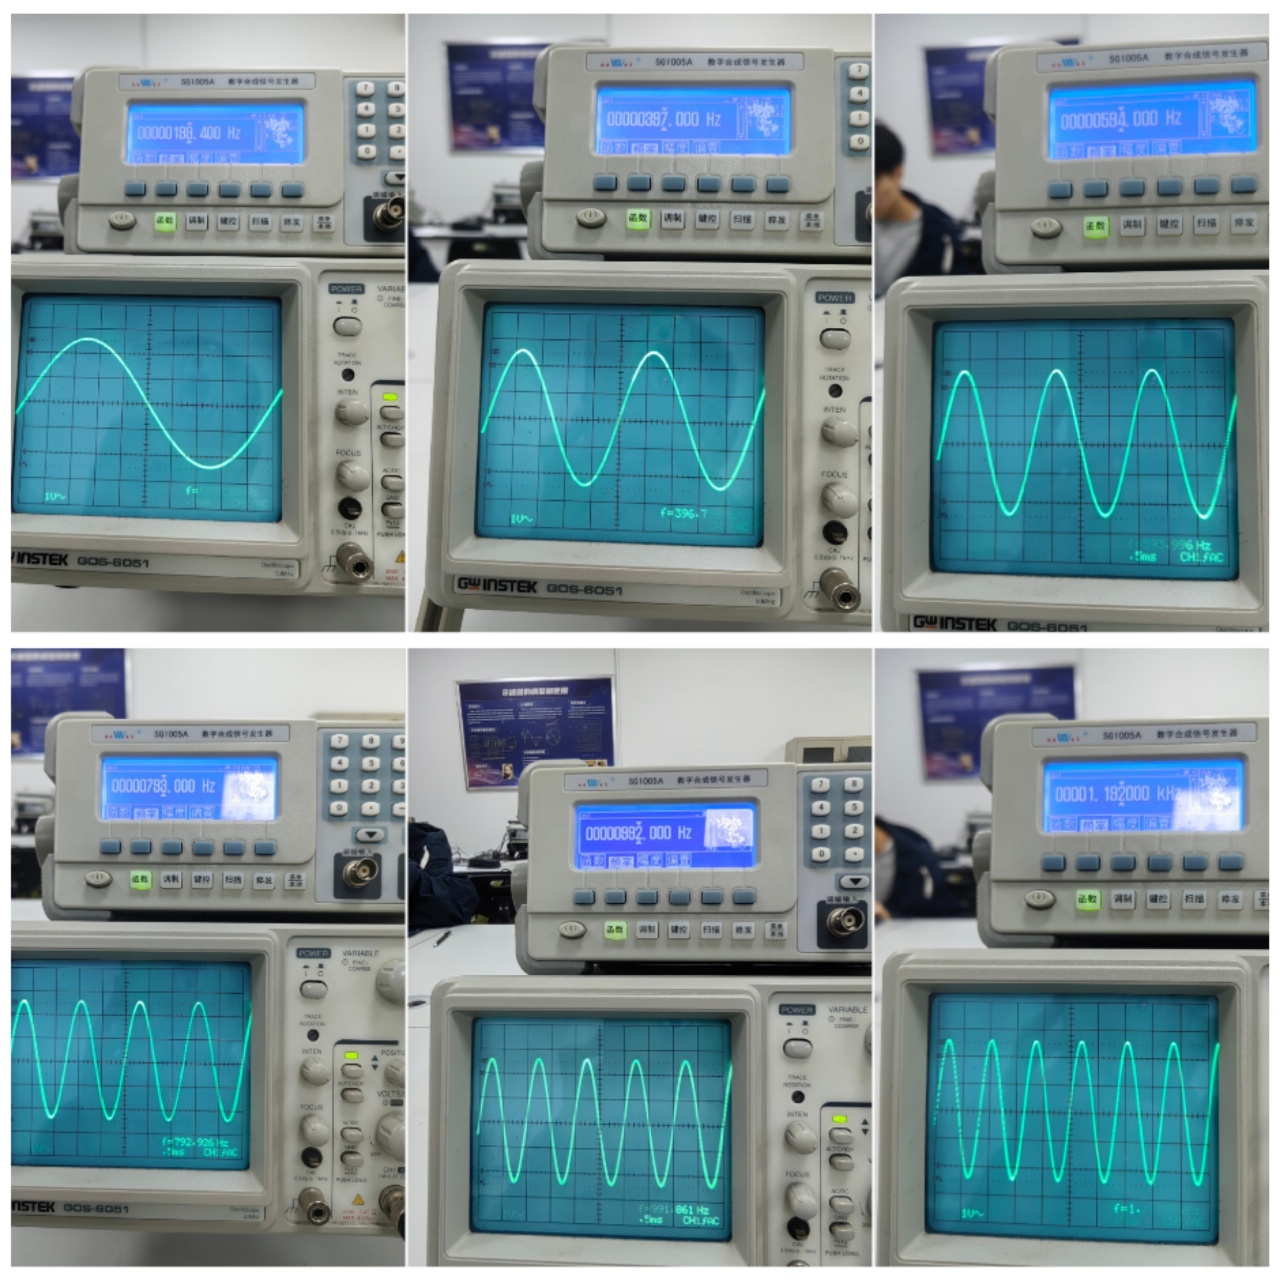
\includegraphics[width=0.9\textwidth]{figure/sum.jpg}
    \caption{比较法验证$f_y=n*f_x$波形1}
    \end{figure}
% 2. 李萨如图形法测量频率
(2)用李萨如图形测量未知信号的频率

信号发生器背后输出的~50Hz的电压，作为fy
\begin{table}[H]
\centering
\caption{李萨如图形法测量频率（参考信号 $f_y = 50$ Hz）}
\begin{tabular}{|c|c|c|c|c|c|c|}
\hline
频率比 $f_y:f_x$ & 1:1 & 1:2 & 1:3 & 2:1 & 2:3 & 3:1 \\ \hline
图形 & 图3& 图4 & 图5 & 图6 & 图7 & 图8 \\ \hline
垂直交点数 $N_y$ & 1 & 2 & 3 & 1 & 3 & 1 \\ \hline
水平交点数 $N_x$ & 1 & 1 & 1 & 2 & 2 & 3 \\ \hline
读出 $f_x$ (Hz) & 49.960 & 100.100 & 150.180 & 25.020 & 74.980 & 16.674 \\ \hline
计算 $f_y$ (Hz) & 49.960 & 50.050 & 50.060 & 50.040 & 49.987 & 50.022 \\ \hline
\end{tabular}
\end{table}

最终结果$\bar{f_y} = \frac{\sum_{i=1}^{6}f_i}{6}=50.020$ Hz，

相对误差$E=\frac{\bar{f_y} - 50}{50} \times 100\% = 0.04\%$

李萨如图图片6张依次附上：
\begin{figure}[H]
    \centering
    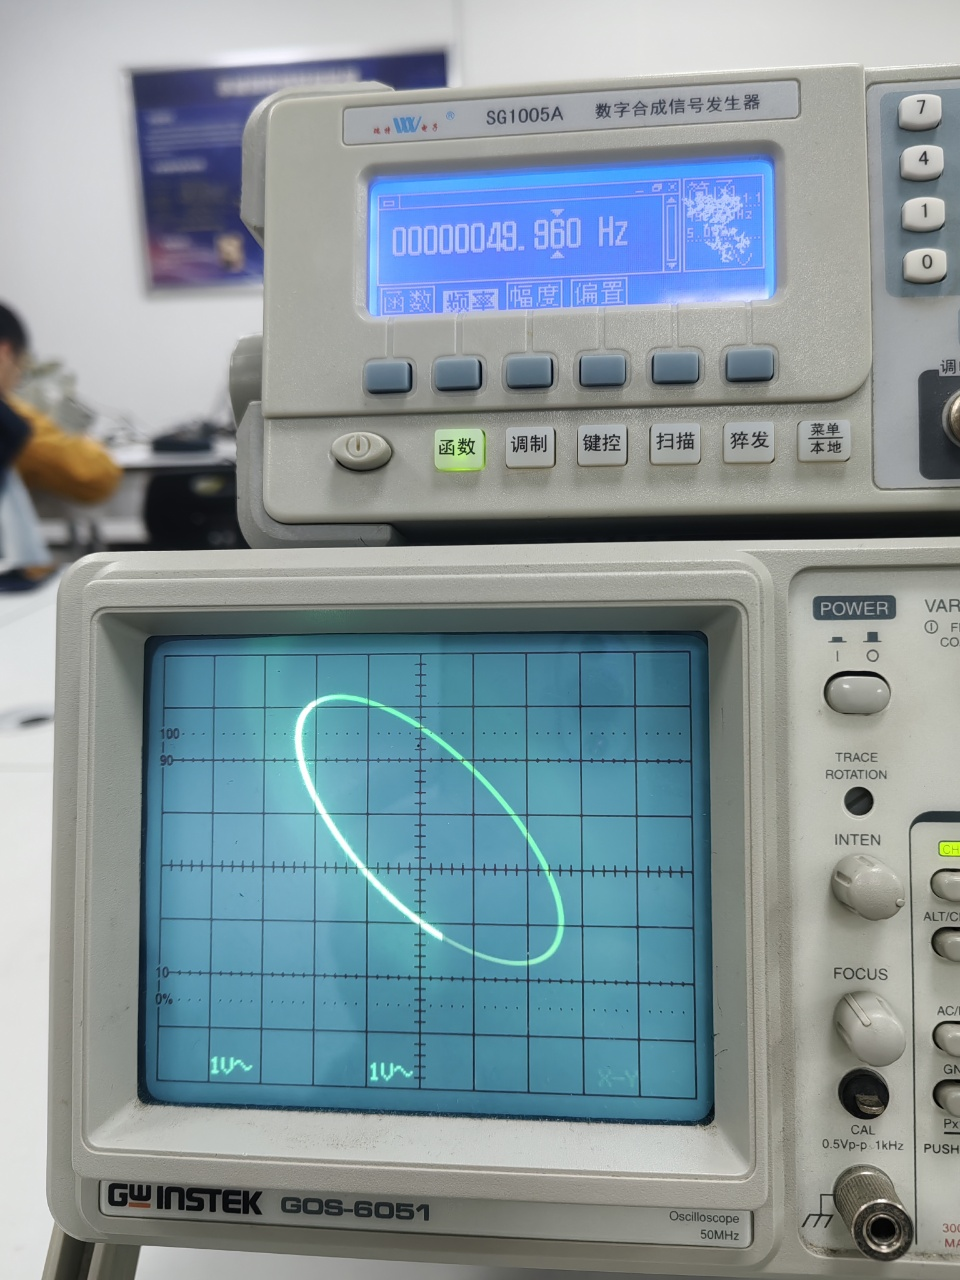
\includegraphics[width=0.9\textwidth]{figure/one_one.jpg}
    \caption{李萨如图形法测量频率波形1}
\end{figure}
\begin{figure}[H]
    \centering
    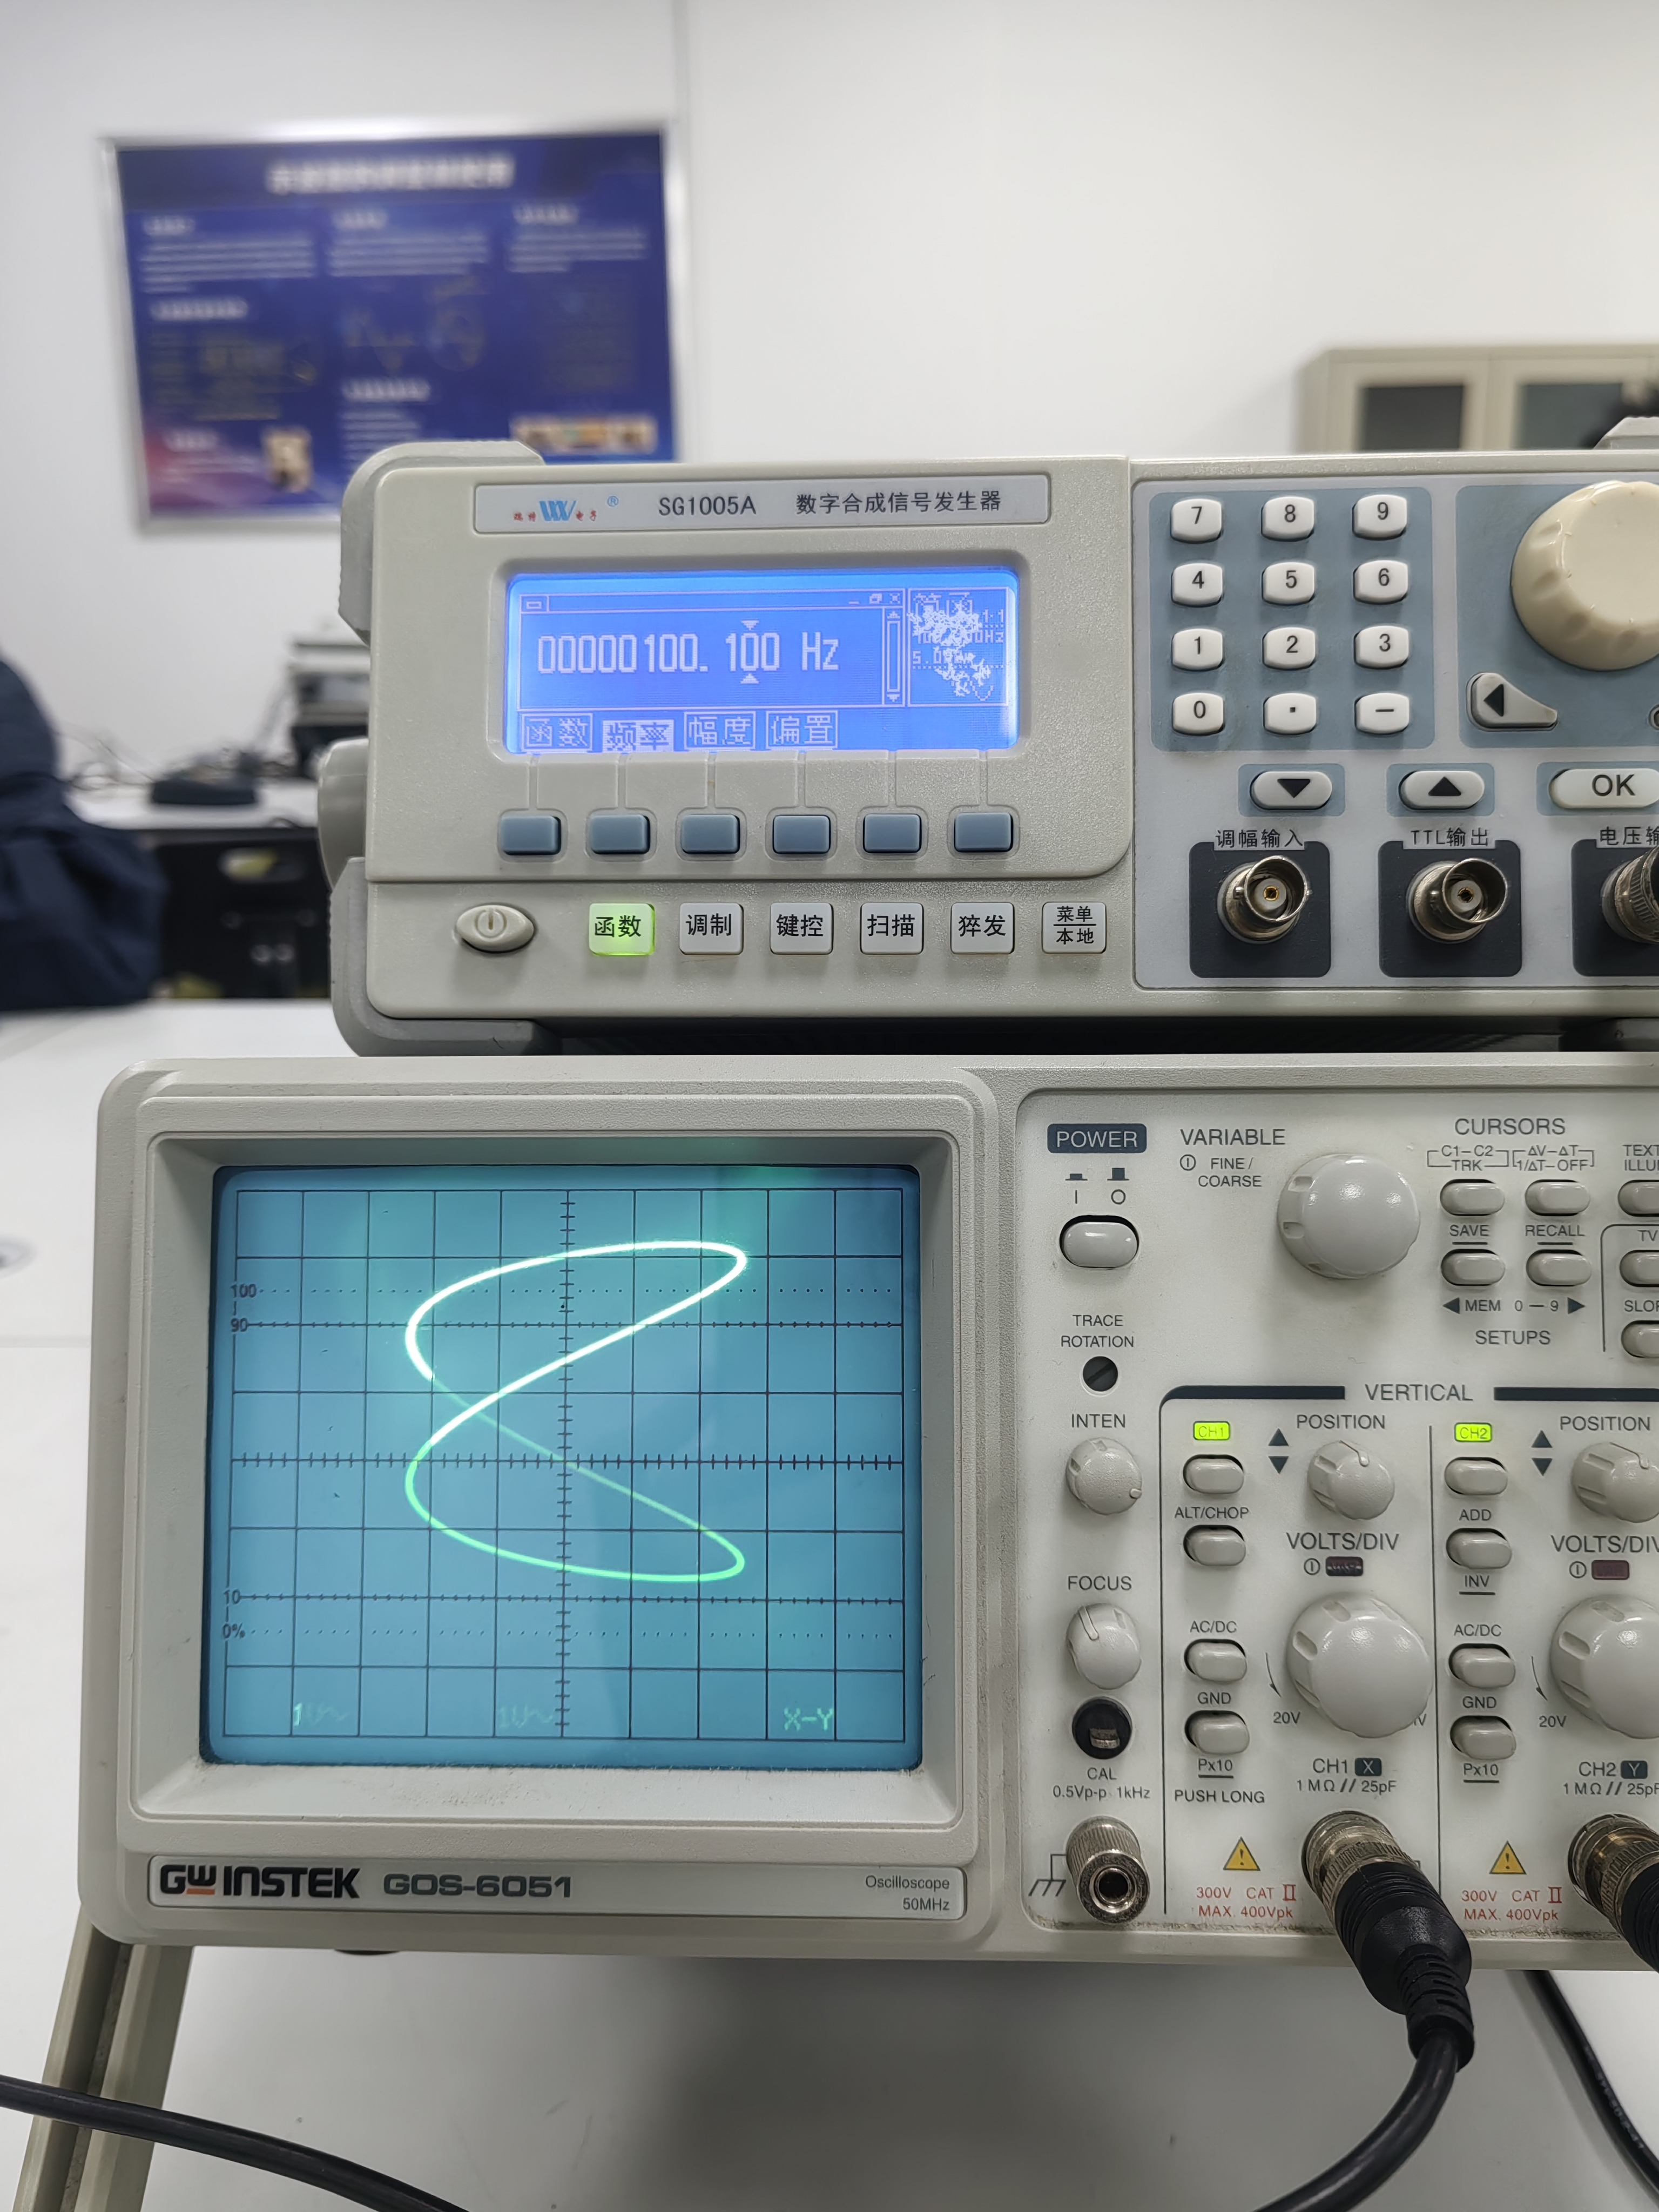
\includegraphics[width=0.9\textwidth]{figure/one_two.jpg}
    \caption{李萨如图形法测量频率波形2}
\end{figure}
\begin{figure}[H]
    \centering
    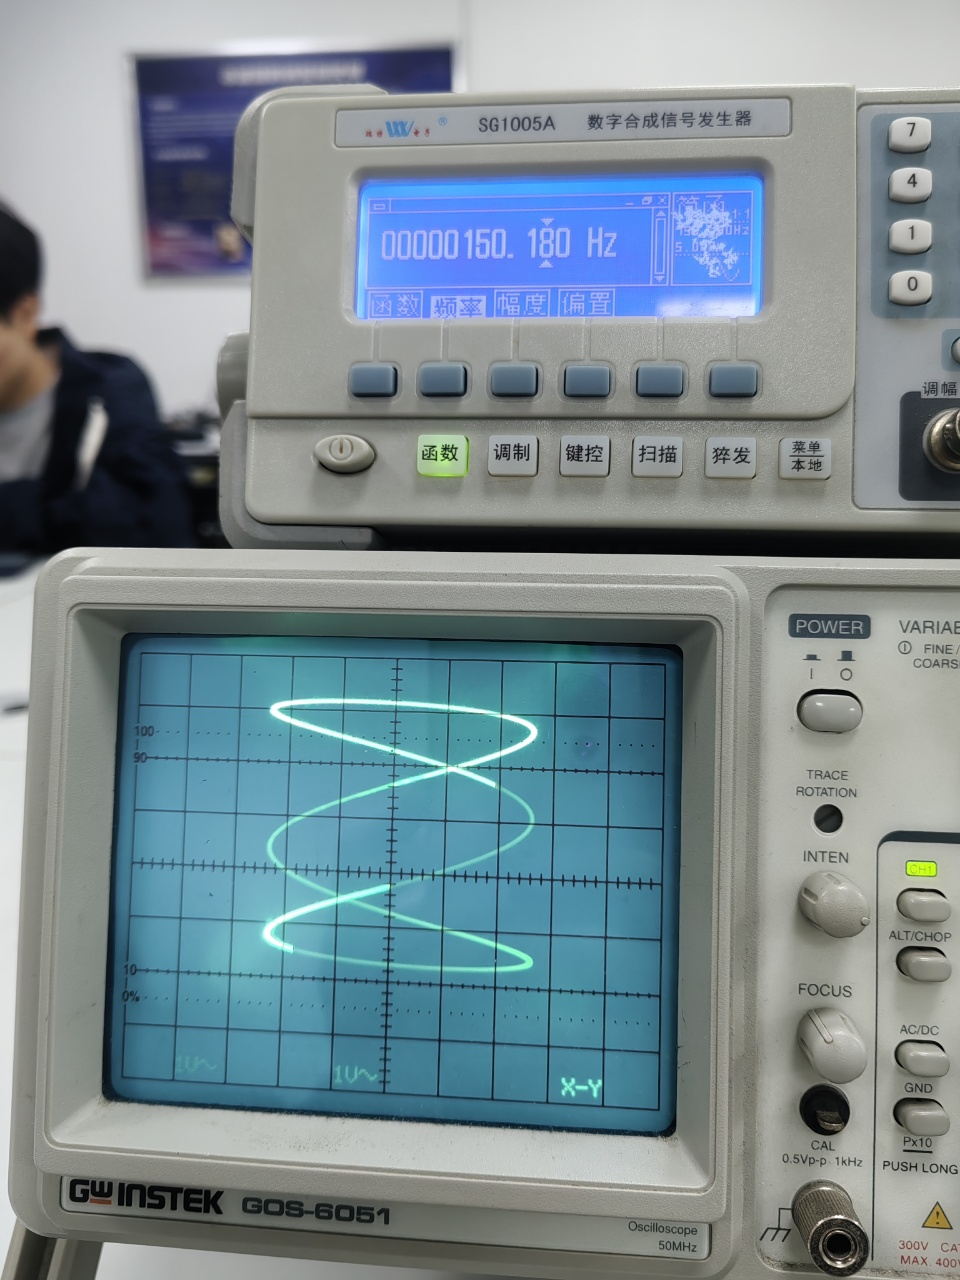
\includegraphics[width=0.9\textwidth]{figure/one_three.jpg}
    \caption{李萨如图形法测量频率波形3}
\end{figure}
\begin{figure}[H]
    \centering
    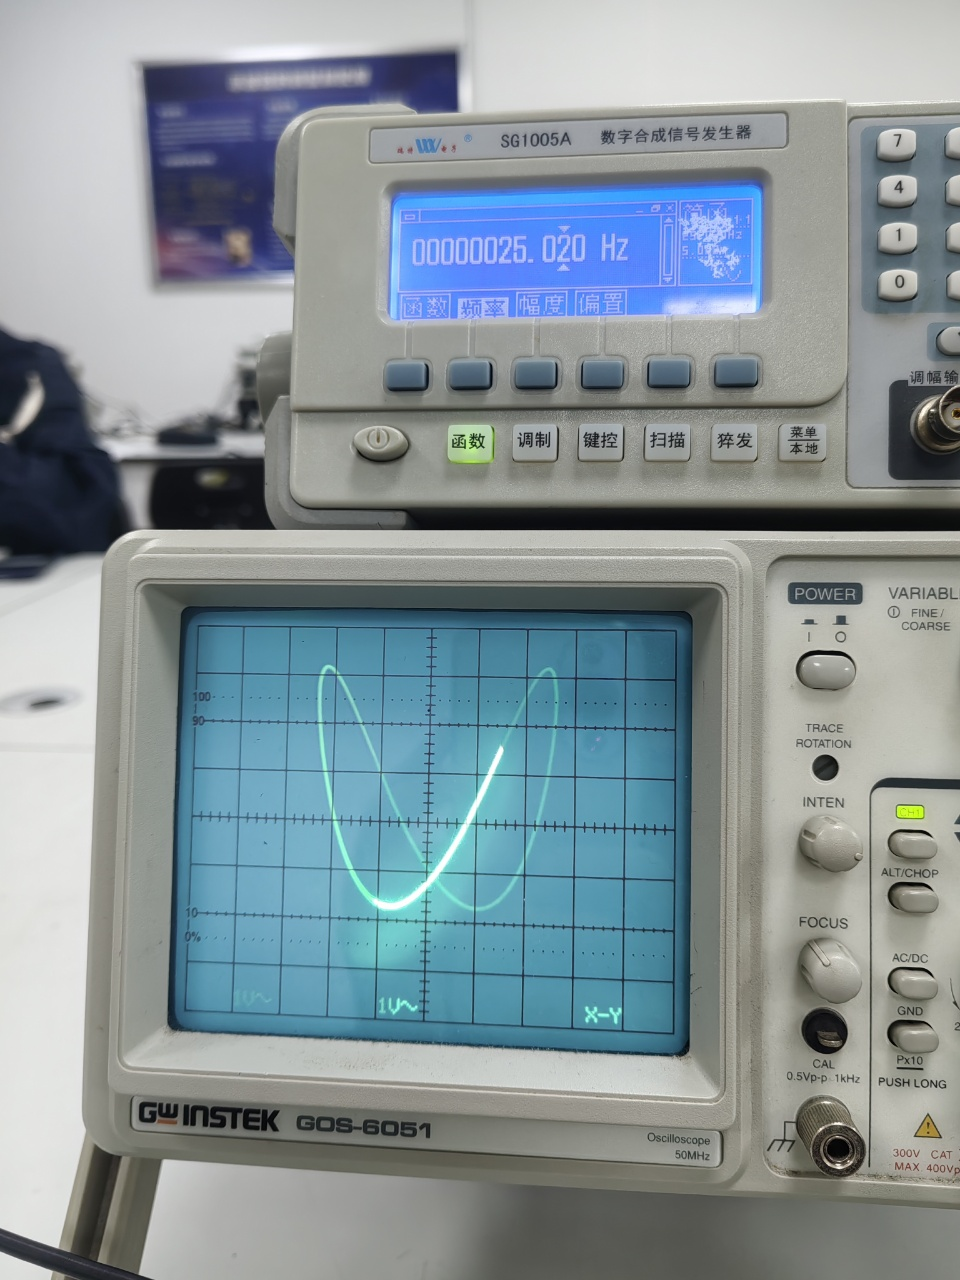
\includegraphics[width=0.9\textwidth]{figure/two_one.jpg}
    \caption{李萨如图形法测量频率波形4}
\end{figure}
\begin{figure}[H]
    \centering
    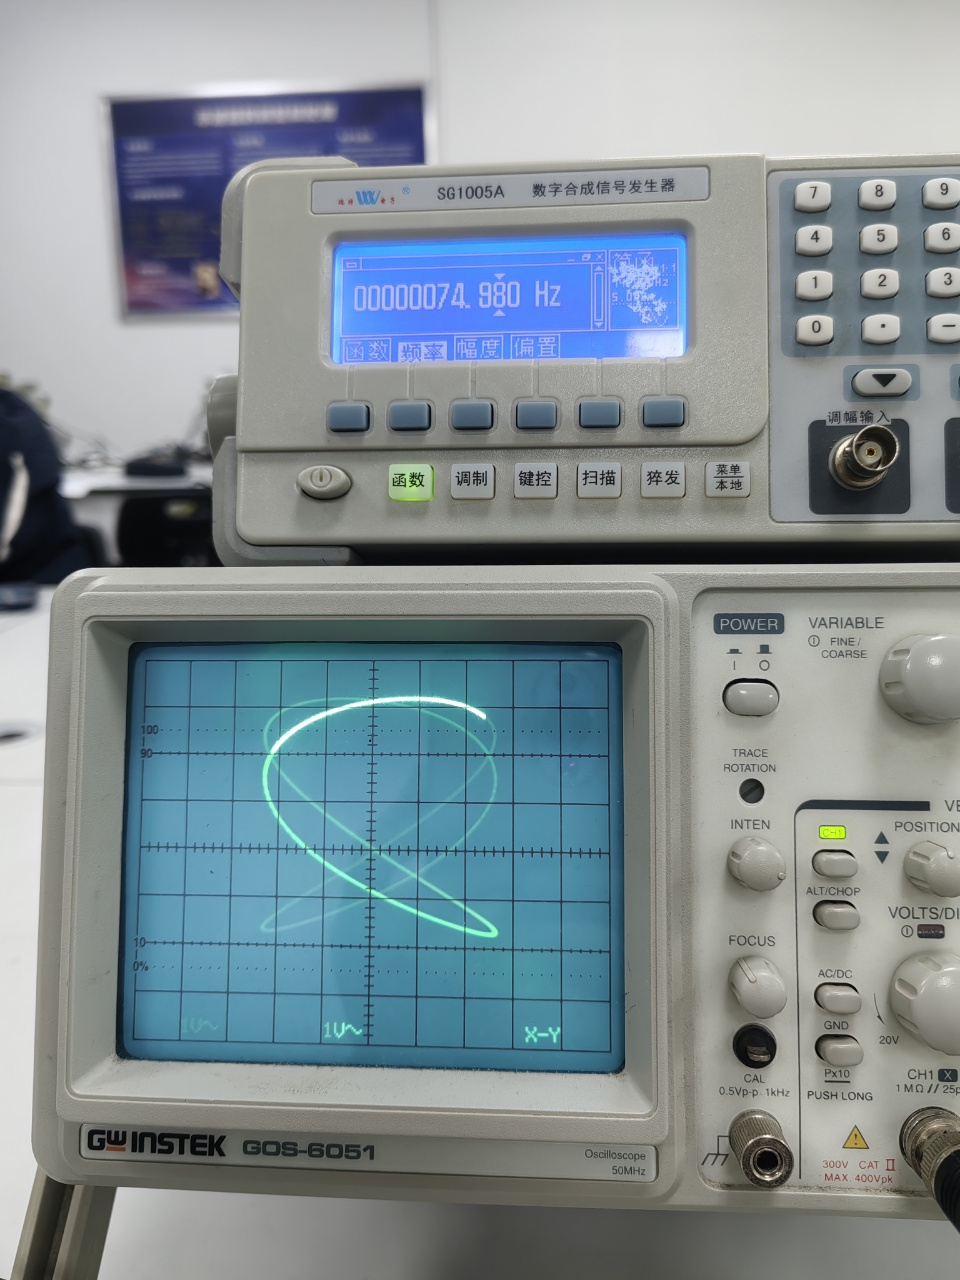
\includegraphics[width=0.9\textwidth]{figure/two_three.jpg}
    \caption{李萨如图形法测量频率波形5}
\end{figure}
\begin{figure}[H]
    \centering
    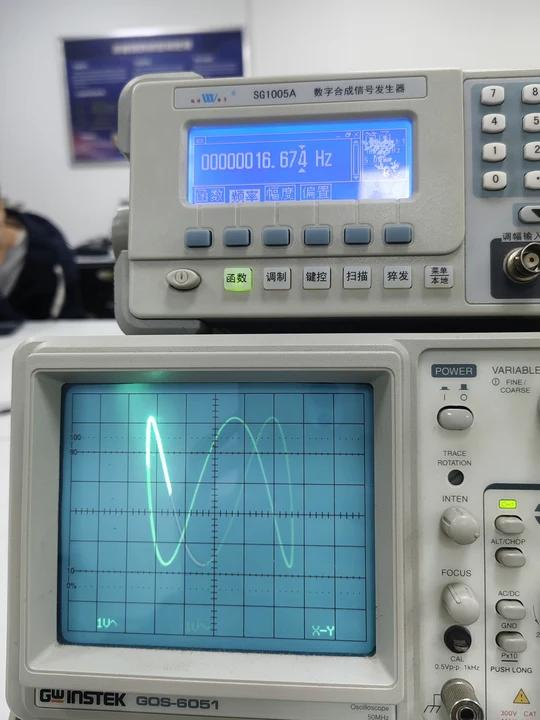
\includegraphics[width=0.9\textwidth]{figure/three_one.jpg}
    \caption{李萨如图形法测量频率波形6}
\end{figure}
(3)二极管正向导通电压的测量
\begin{table}[H]
\centering
\caption{二极管正向导通电压测量（光标法）}
\begin{tabular}{|c|c|}
\hline
输入电压峰峰值 $U_{1P-P}$ (V) & 4.96   \\ \hline
输出半波电压峰值 $U_{2P}$ (V) & 1.76   \\ \hline
正向导通电压 $U_{\text{导通}}$ (V) &  0.72  \\ \hline
\end{tabular}
\end{table}

$U_{\text{导通}} =\frac{1}{2} U_{1P-P} - U_{2P} = 2.48 - 1.76 = 0.72$ V

示波器图形如下：
\begin{figure}[H]
    \centering
    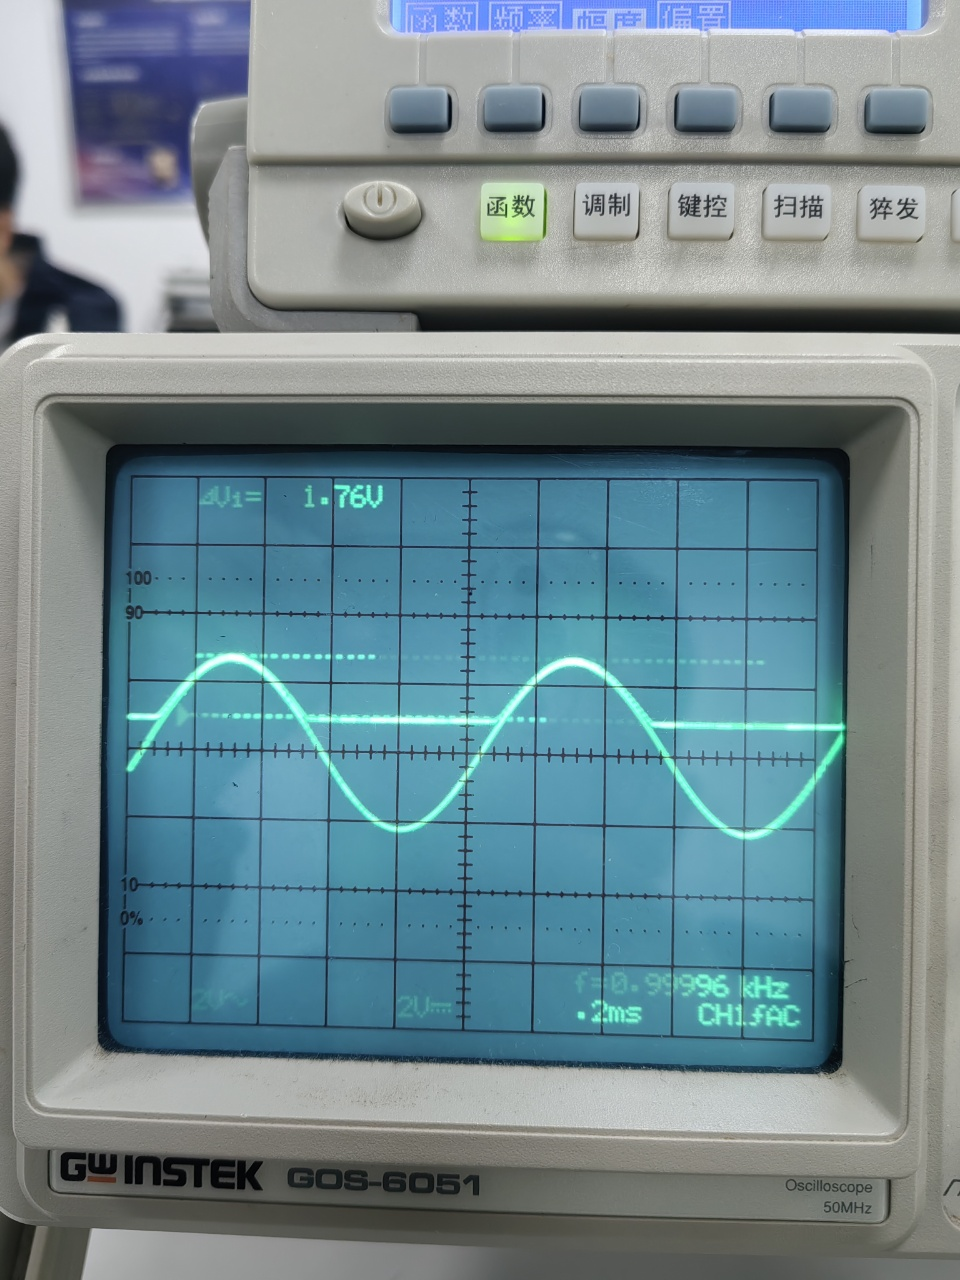
\includegraphics[width=0.6\textwidth]{figure/di.jpg}
    \caption{二极管正向导通电压测量波形}
    \end{figure}

(4)RC电路输入输出波形相位差的测量
\begin{table}[H]
\centering
\caption{RC电路相位差测量（$R = 750 \Omega$, $C = 0.47\mu F$ F, 输入频率 = 1kHz）}
\begin{tabular}{|c|c|c|}
\hline
波形时间差 $\Delta t$ (s) & 周期 $T$ (s) & 相位差 $\Delta \phi$  \\ \hline
0.184ms & 1.000ms &  $66.24^\circ$\\ \hline
\end{tabular}
\end{table}
$\Delta \phi = \frac{\Delta t}{T} \times 360^\circ=66.24^\circ$

示波器图形如下：
\begin{figure}[H]
    \centering
    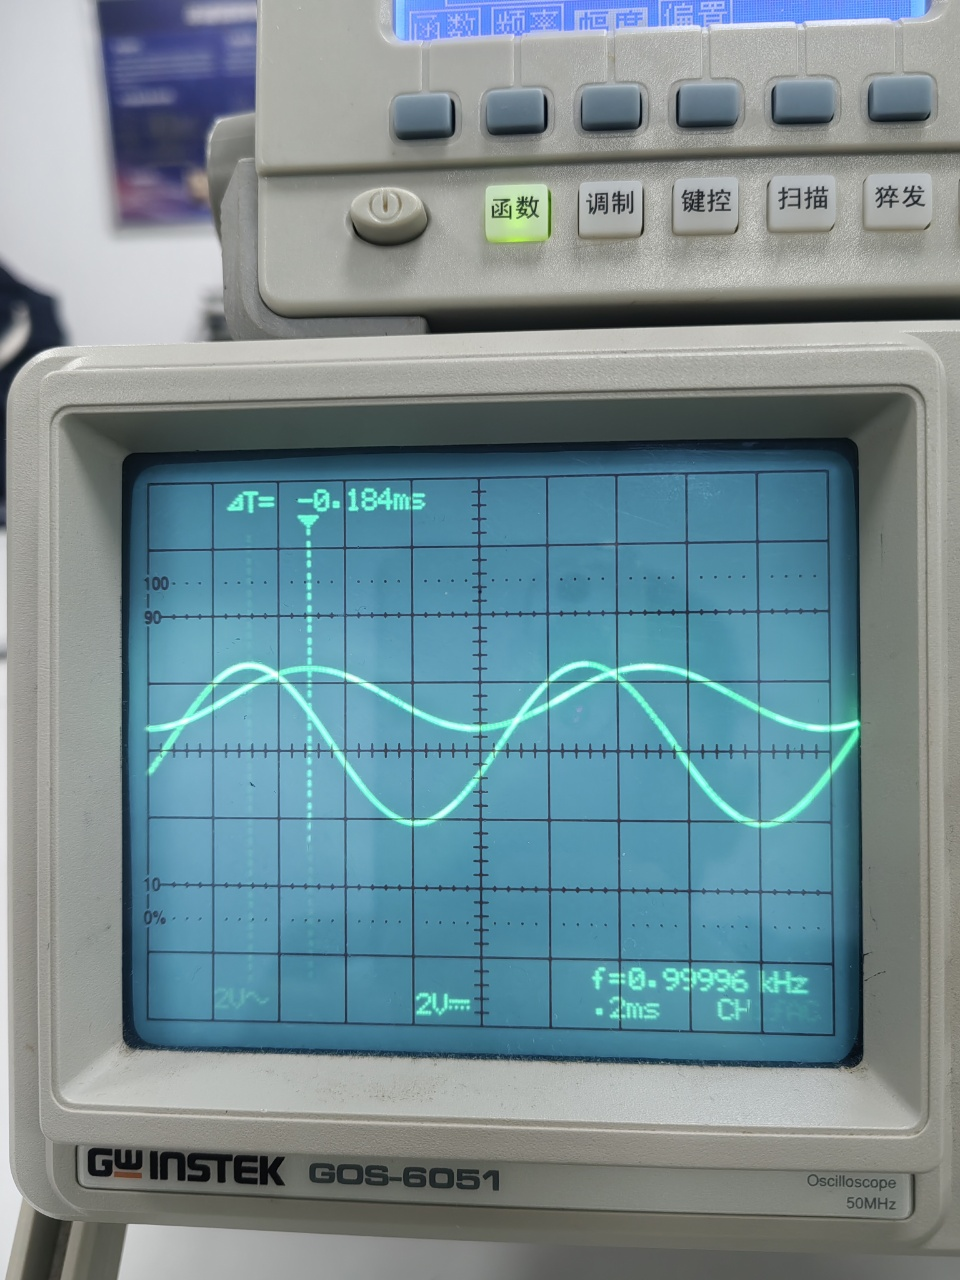
\includegraphics[width=0.6\textwidth]{figure/cap.jpg}
    \caption{RC电路输入输出波形}
    \end{figure}
\subsection{误差分析}
(1)比较验证法的不确定度计算如下：
\begin{align*}
u_A &= \sqrt{\frac{\sum (f_i - \bar{f})^2}{n(n-1)}} \\
&= \sqrt{\frac{(199.400-198.536)^2 + \cdots + (198.667-198.536)^2}{6 \times 5}} \\
&= 0.228 \text{ Hz}
\end{align*}
最终结果：$\bar{f_x} = (198.536 \pm 0.228)$ Hz，相对误差 $E = 0.7\%$。

(2)李萨如图形法测量频率的不确定度计算如下：
\begin{align*}
u_A &= \sqrt{\frac{\sum (f_{y,i} - \bar{f_y})^2}{n(n-1)}} \\
&= \sqrt{\frac{(49.960-50.020)^2 + \cdots + (50.022-50.020)^2}{6 \times 5}} \\
&= 0.018 \text{ Hz}.
\end{align*}
最终结果：$f_y = (50.020 \pm 0.018)$ Hz，相对误差 $E = 0.04\%$。

实验误差来源分析：
\begin{itemize}
    \item 示波器读数误差：示波器的刻度有限，读数时存在一定的主观误差。
    \item 信号源稳定性：信号源频率和幅度的微小波动会影响测量结果。
    \item 环境干扰：实验环境中的电磁干扰可能会影响示波器的显示效果。
    \item 测量方法局限性：不同测量方法对结果的敏感度不同，可能导致误差。
    \item  仪器校准：示波器和信号源的校准状态会影响测量精度。
    \item 连接线质量：使用的连接线质量不佳可能引入额外的阻抗和噪声。
    \item 李萨如图像稳定性：李萨如图形的稳定性对频率比测量有较大影响，抖动会导致读数不准确。实验要求调节李萨如图形尽量使之稳定时进行频率读取，但是实际操作时难免存在一定抖动，难以做到完全稳定。
\end{itemize}
\subsection{实验探讨}
通过示波器实验掌握了波形测量、频率分析和相位差测量方法。发现李萨如图形的稳定性对频率比测量至关重要。
\section{思考题}

    \xiaosi （解答教材或讲义或老师布置的思考题，10分）
    
1.示波器的主要结构与各部分的作用是什么？示波器为什么能显示被
测信号的波形？

示波器的主要结构包括阴极射线管（CRT）、垂直放大器、水平放大器、扫描发生器、触发电路和电源等部分。阴极射线管是示波器的核心，用于显示波形；垂直放大器放大被测信号，使其在垂直方向上产生适当的偏转；水平放大器控制水平扫描信号，使电子束在水平方向上移动；扫描发生器产生锯齿波信号，控制电子束的水平扫描；触发电路确保扫描与被测信号同步，使波形稳定显示。示波器能显示被测信号的波形是因为电子束在垂直方向上受被测信号电压的控制，在水平方向上受扫描电压的控制，两者共同作用使电子束在荧光屏上描绘出信号的波形。

2.在观察李萨如图形时为什么总是不断的来回翻动，翻动的快慢是受
哪种因素所影响

在观察李萨如图形时，图形不断翻动是因为两个信号的频率比不是严格的整数比或相位差在不断变化。翻动的快慢受两个信号的频率差影响，频率差越小，翻动越慢；频率差越大，翻动越快。当两个信号的频率比为严格的整数比且相位差固定时，李萨如图形会稳定显示。

3. 切实理解示波器同步的概念，如果发生波形左移或右移时应该如何
调整才能使其稳定下来？

示波器同步的概念是指通过触发电路使扫描信号的起始点与被测信号的特定点（如上升沿或下降沿）保持一致，从而使波形稳定显示。如果发生波形左移或右移，说明触发点与扫描信号的同步不稳定。可以通过调整触发电平或触发极性（上升沿或下降沿）来使波形稳定。具体方法是：调节触发电平旋钮，使触发电平位于被测信号的适当位置；或调整触发极性，选择与被测信号变化方向一致的触发边沿。此外，还可以调整扫描时间因数，使扫描速度与被测信号频率匹配，从而获得稳定的波形显示。

\sihao\textbf{注意事项：}
\xiaosi
\begin{enumerate}
    \item 用PDF格式上传“实验报告”，文件名：学生姓名+学号+实验名称+周次。
    \item  “实验报告”必须递交在“学在浙大”的本课程的对应实验项目的“作业”模块内。
    \item  “实验报告”成绩必须在“浙江大学物理实验教学中心网站”-“选课系统”内查询。
    \item 教学评价必须在“浙江大学物理实验教学中心网站”-“选课系统”内进行，学生必须进行教学评价，才能看到实验报告成绩，教学评价必须在本次实验结束后 3 天内进行。
\end{enumerate}

\vspace{1cm}
\xiaosi\centering \textbf{浙江大学物理实验教学中心制}

\end{document}